\begin{figure}[h]
	\centering
	\begin{tikzpicture}[x=2cm, every edge/.style={draw,postaction={decorate,decoration={markings,mark=at position 1.0 with {\arrow[scale=2]{>}}}}}]
		\node[rectangle] (c2) at (1,2) [label=left:$c_{2}:$]{
			\begin{tikzpicture}[x=1cm]
				\draw (0,0)--(1,0)--(1,1)--(0,1)--cycle;
				\draw (.5,0)--(.5,.5)--(.5,1);
				\draw (0,.5)--(.5,.5)--(1,.5);
				\draw (.25,.25) circle (3pt);
				\filldraw (.25,.75) circle (3pt);
			\end{tikzpicture}		
		};
		\node[rectangle] (c1) at (0,0) [label=below:$c_{1}$]{
			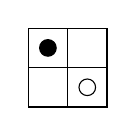
\begin{tikzpicture}[x=1cm]
				\draw (0,0)--(1,0)--(1,1)--(0,1)--cycle;
				\draw (.5,0)--(.5,.5)--(.5,1);
				\draw (0,.5)--(.5,.5)--(1,.5);
				\draw (.75,.25) circle (3pt);
				\filldraw (.25,.75) circle (3pt);
			\end{tikzpicture}
		};
		\node[rectangle] (c4) at (1,0) [label=below:$c_{4}$]{
			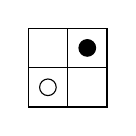
\begin{tikzpicture}[x=1cm]
				\draw (0,0)--(1,0)--(1,1)--(0,1)--cycle;
				\draw (.5,0)--(.5,.5)--(.5,1);
				\draw (0,.5)--(.5,.5)--(1,.5);
				\draw (.25,.25) circle (3pt);
				\filldraw (.75,.75) circle (3pt);
			\end{tikzpicture}
		};
		\node[rectangle] (c8) at (2,0) [label=below:$c_{8}$]{
			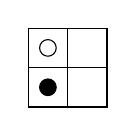
\begin{tikzpicture}[x=1cm]
				\draw (0,0)--(1,0)--(1,1)--(0,1)--cycle;
				\draw (.5,0)--(.5,.5)--(.5,1);
				\draw (0,.5)--(.5,.5)--(1,.5);
				\draw (.25,.75) circle (3pt);
				\filldraw (.25,.25) circle (3pt);
			\end{tikzpicture}
		};
		\path
			(c2) edge (c1)
			(c2) edge (c4)
			(c2) edge (c8)
		;
	\end{tikzpicture}
	\caption{Transformations of the configuration $c_{2}$}
\end{figure}